\documentclass[a4paper,12pt]{article}
\usepackage[utf8]{inputenc}
\usepackage[spanish]{babel}
\usepackage{microtype}
 
\usepackage{graphicx}
\usepackage{wrapfig}
 
\usepackage{amssymb}
\usepackage{amsmath} %For being able to make comments inside the formulas as normal text
\usepackage{amsthm}

\usepackage{cancel} %in the preamble gives you four different modes of striking through

\usepackage[a4paper, inner= 2cm, outer= 2cm,
top= 2cm, bottom= 2cm]{geometry}
\usepackage{fancyhdr}
\usepackage{animate}

\title{Taller 1}
\author{David Alsina, Jairo Gudiño, Juan Ávila}
\date{Enero 2021}

\usepackage[dvipsnames]{xcolor}
\definecolor{blueMacc}{RGB}{61, 160, 250}

\begin{document}

    \begin{figure}[ht]
         \centering
		 
\includegraphics[width = \linewidth]{./header.png}
         \maketitle
    \end{figure}

    \begin{enumerate}
        \item Muestre que $Re(iz)$ = -$Im(z)$ para todo número complejo z.
        
        \item Sea k un número entero. Muestre que:
            
            \begin{enumerate}
                \item $i^{4k} = (i^{4})^{k} = (1)^{k} = 1$
                \item $i^{4k + 1} = (i^{4})^{k} \cdot i^{1} = (1)^{k} \cdot i^{1} = i$
            \end{enumerate}
        
        \item Encuentre el valor de las siguientes potencias de i.
        
                \item 

        \item Encuentre $z_{1} y z_{2}$ tal que se satisfaga el siguiente sistema de ecuaciones:

            \begin{equation}
                (1 - i)z_{1} + 3z_{2} = 2 - 3i  
            \end{equation}
                
            %solucion de eqn
            \begin{eqnarray*}
                \colorbox{blueMacc}{$z_{2}$} = \frac{2 - 3i - (1 - i)z_{1}}{3}
            \end{eqnarray*}

            \begin{equation}
                iz_{1} + (1 + 2i)z_{2} = 1 
            \end{equation}
            
            \begin{equation*}
                \colorbox{blueMacc}{$z_{1}$}=\frac{1-(1+2 i) z_{2}}{i}=-i+(1+2 i) z_{2}
            \end{equation*}

            \begin{center}
                \textbf{Ahora evaluando $z_{1}$ en $z_{2}$}:             
            \end{center}

            %solucion de eqn
            \begin{align*}
                z_{2} &=\frac{2}{3}-i-\left[\frac{(1-i) \cdot\left(-i+(1+2 i) z_{2} i\right)}{3}\right] \\
                &=\frac{2}{3}-i-\left[\frac{-i+z_{2} i-2 z_{2}-1+z_{2}+2 i z_{2}}{3}\right] \\
                &=\frac{2}{3}-i-\left[\frac{-i+3 i z_{2}-z_{2}-1}{3}\right]=1-\frac{2}{3} i-i z_{2}+\frac{z_{2}}{3}\\
                z_{2}\left(\frac{2}{3}+i\right) &=1-\frac{2}{3} i \\
                \colorbox{blueMacc}{$z_{2}$} &=\frac{1-\frac{2}{3} i}{\frac{2}{3}+i}= -i
            \end{align*}
            
            \begin{center}
                \textbf{Finalmente evaluando el valor de $z_{2}$ en $z_{1}$:}
                \begin{align*}
                    (1 - i)z_{1} + \cancel{3(-i)} &= 2 - \cancel{3i}\\
                    \colorbox{blueMacc}{$z_{1}$} &= \frac{2}{1 - i} = 1 + i\\
                \end{align*}
            \end{center}
            
        \item Encuentre todas las soluciones para $z^{4} - 16 = 0$
        
              (i) Soluciones de forma algebraica
              
            \begin{align*}
                z^{4} = 16\\
                z^{4/4} = 16^{1/4}
            \end{align*}
            
            En consecuencia, $z=2$ y $z=-2$
            
            (ii) Soluciones de forma polar
            
            Como $z^{4} = r^{4}cis(4\theta) = 16cis(4\theta) = 16cis(0) = 16$, al ser representarse geométricamente $z^{4}$ como un vector con ángulo 0, por definición también tiene un ángulo igual a $2\pi$, de manera que $4\theta = 2\pi$ y por lo tanto $\theta = \pi/2$, de manera que $z = 2cis(\theta) = 2cis(\pi/2) = 2i$. Siguiendo esta misma idea, $z^{4}$ también tiene un ángulo igual a $4\pi$, de manera que $4\theta = 4\pi$ y por lo tanto $\theta = \pi$, y en consecuencia, $z = 2cis(\theta) = 2cis(\pi) = -2i$. En consecuencia, $z=2i$ y $z=-2i$.

        
        \item
            
        \item Sea $z = 3$ $-2i$. Grafique los puntos z, -z, \={z}, -\={z}  en el plano complejo.
        La gráfica de z, -z, \={z}, -\={z} es:
            
            \begin{center}
                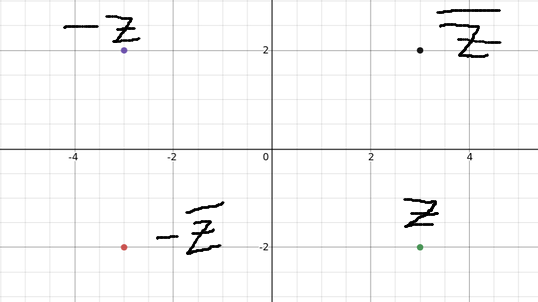
\includegraphics[width= 0.6\linewidth]{taller1_pto8.png}\\    
                \textit{Note como multiplicar por -1 produce una rotación de 180°, mientras que el complemento produce una reflexión sobre la recta real.}
            \end{center}
            
        \item 
        
        \item 
        
        \item Muestre lo siguiente:
            $arg(z_{1}z_{2}z_{3}) = arg(z_{1}) + arg(z_{2}) + arg(z_{3})$
    
            \begin{align*}
                arg(z_{1}z_{2}z_{3}) = arg((z_{1}z_{2})z_{3}) &= arg(r_{1}r_{2}\cdot cis(\theta_{1} + \theta_{2})z_{3})\\
                &= arg( r_{1}r_{2}\cdot cis(\theta_{1} + \theta_{2})\cdot r_{3} \cdot cis(\theta_{3}))\\
                &= arg( r_{1}r_{2}r_{3} \cdot cis(\theta_{1} + \theta_{2}) \cdot cis(\theta_{3}))\\
                &= arg( r_{1}r_{2}r_{3} \cdot cis(\theta_{4})cis(\theta_{3})); \;\; \text{donde $\theta_{1}+\theta_{2} = \theta_{4}$}
            \end{align*}

            \begin{center}
                siguiendo un argumento análogo al visto para $arg(z_{1}z_{2}) = arg(z_{1})+arg(z_{2})$ se tiene: 
            \end{center}
            \begin{align*}
                &= arg( r_{1}r_{2}r_{3} cis(\theta_{4}+\theta_{3}))\\
                &= arg( r_{1}r_{2}r_{3} cis(\theta_{1}+\theta_{2} + \theta_{3}))\\
                &= arg(r_{5}\cdot cis(\theta_{5}))
                \text{\;donde\; $r_{5} = r_{1}r_{2}r_{3}$} \text{\; y $\theta_{5} = \theta_{1}+\theta_{2}+\theta_{3}$}\\
                &= \theta_{5} = \theta_{1} + \theta_{2} + \theta_{3}
            \end{align*}
            
          
        
        Muestre lo siguiente:
            $arg(z_{1}\bar{z_{2}}) = arg(z_{1}) - arg(z_{2})$
        
        Dado que $\bar{z_{2}}$ hace referencia geométricamente a un vector que es reflejo de $z_{2}$ en el eje X, entonces su ángulo se puede calcular como $2\pi - \theta_{2}$, por lo que
        
            \begin{align*}
                z_{1}\bar{z_{2}} = |z_{1}||\bar{z_{2}}|cis(\theta_{1} + 2\pi - \theta_{2}) &= |z_{1}||z_{2}|\left[cos(\theta_{1} + 2\pi)+isin(\theta_{1} + 2\pi)\right]\left[cos(-\theta_{2})+isin(-\theta_{2})\right]\\
                &= |z_{1}||z_{2}|\left[cos(\theta_{1})+isin(\theta_{1})\right]\left[cos(-\theta_{2})+isin(-\theta_{2})\right]\\
                &= |z_{1}||\bar{z_{2}}|cis(\theta_{1} - \theta_{2})\\
            \end{align*}
            
        En consecuencia,
        
            \begin{align*}
                arg(z_{1}\bar{z_{2}}) = \theta_{1} - \theta_{2}\\
            \end{align*}
            
        \item Para cada uno de los siguientes números calcule sus raı́ces quintas. Determine y grafique el polígono que genera, y calcule la longitud de sus aristas. ¿En ambos casos son las aristas iguales? Justifique la respuesta:
        
        \begin{enumerate}
            \item $z_{0}=-1$\\
            Podemos representar en $z_0$ como $e^{i\frac{3\pi}{2}}$. Luego, calculamos sus raíces de la siguiente manera: 
            $$-1^{\frac{1}{5}} = 1^{\frac{1}{5}} e^{\frac{i\left(\frac{3\pi}{2}+2\pi  k\right)}{5}}, \quad \textrm{siendo}\quad k=0, 1,2,3,4$$ 
            Sus cinco raíces serían:\\
            \begin{itemize}
                \item $ e^{\frac{i\left(\frac{3\pi}{2}\right)}{5}} = \cos \left( \frac{3\pi}{10}\right) +i \sin \left( \frac{3\pi}{10}\right)$
                \item $ e^{\frac{i\left(\frac{3\pi}{2}+2\pi\right)}{5}} = \cos \left( \frac{7\pi}{10}\right) +i \sin \left( \frac{7\pi}{10}\right)$
                \item $ e^{\frac{i\left(\frac{3\pi}{2}+4\pi\right)}{5}} = \cos \left( \frac{11\pi}{2}\right) +i \sin \left( \frac{11\pi}{2}\right)$
                \item $ e^{\frac{i\left(\frac{3\pi}{2}+6\pi\right)}{5}} = \cos \left( \frac{15\pi}{2}\right) +i \sin \left( \frac{15\pi}{2}\right)$
                \item $ e^{\frac{i\left(\frac{3\pi}{2}+8\pi\right)}{5}} = \cos \left( \frac{19\pi}{10}\right) +i \sin \left( \frac{19\pi}{10}\right)$
            \end{itemize}
            \textbf{Gráfica}
            \begin{center}
            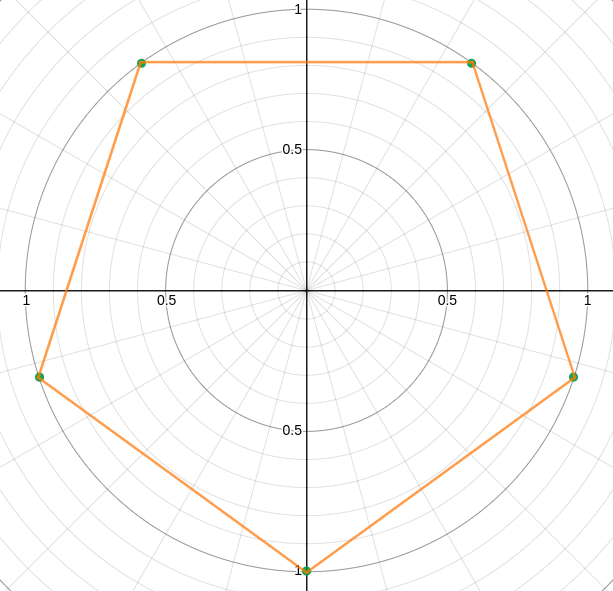
\includegraphics[scale=0.4]{16-a.png}  
            \end{center}
             
            \item $z_0 = 1+i$\\
            Representado $z_0$ de otra manera, tenemos que $z_0= \sqrt{2}e^{i\frac{1}{4}\pi}$. Así pues, sus raíces quintas viened dadas por:\\
            $$(1+i)^{\frac{1}{5}} = \sqrt{2}e^{i\left(\frac{1}{4}\pi + 2\pi k\right)\frac{1}{5}}, \quad \textrm{siendo} \quad k = 0,1,2,3,4$$\\
            De este modo, sus raíces serían:
            \begin{itemize}
                \item $\sqrt{2}e^{i\left(\frac{1}{4}\pi \right)\frac{1}{5}} = \sqrt{2}\left( \cos\left(\frac{1}{20}\pi\right) + i \sin\left({\frac{1}{20}\pi}\right)\right)$
                \item $\sqrt{2}e^{i\left(\frac{1}{4}\pi + 2\pi \right)\frac{1}{5}} = \sqrt{2}\left( \cos\left(\frac{9}{20}\pi\right) + i \sin\left({\frac{9}{20}\pi}\right)\right)$
                \item $\sqrt{2}e^{i\left(\frac{1}{4}\pi + 4\pi \right)\frac{1}{5}} = \sqrt{2}\left( \cos\left(\frac{17}{20}\pi\right) + i \sin\left({\frac{17}{20}\pi}\right)\right)$
                \item $\sqrt{2}e^{i\left(\frac{1}{4}\pi + 8\pi \right)\frac{1}{5}} = \sqrt{2}\left( \cos\left(\frac{5}{4}\pi\right) + i \sin\left({\frac{5}{4}\pi}\right)\right)$
                \item $\sqrt{2}e^{i\left(\frac{1}{4}\pi + 2\pi \right)\frac{1}{5}} = \sqrt{2}\left( \cos\left(\frac{33}{20}\pi\right) + i \sin\left({\frac{33}{20}\pi}\right)\right)$
            \end{itemize}
            \textbf{Gráfica}
            \begin{center}
            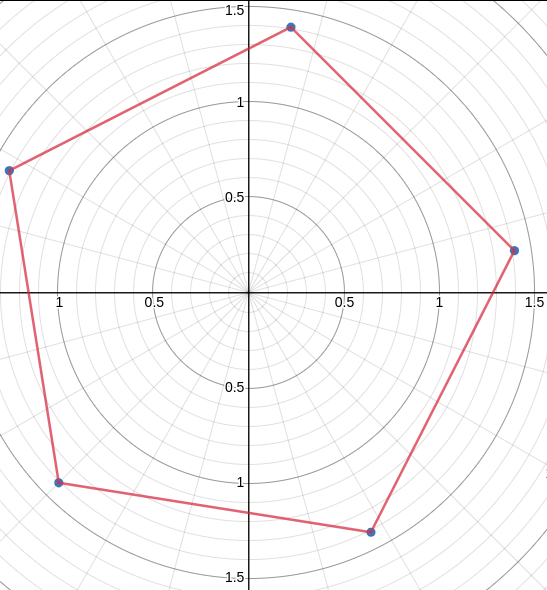
\includegraphics[scale=0.4]{16-b.png}  
            \end{center}
             
        \end{enumerate}
        \textbf{Conclusión aristas}
        \\Las aristas de los polígonos miden en cada uno de ellos igual. Podemos verlo de dos maneras: la primera es que todas las raíces son un número complejo con la el mismo módulo, también podemos apreciar en la gráfica que los puntos forman un polígono regular circunscrito en una circunferencia cuyo radio es el módulo del número complejo al cual se le saca la raíz.
    \end{enumerate}
\end{document}

